% !TEX root = Master.tex

Simple maximum likelihood estimation based on the log-sales of the marginals allow us to estimate the exGaussian distribution parameters. \autoref{fig:kcc_2_marginal} describes how the histogram of the data match to the theoretical density of an exGaussian distribution considering the estimated parameter values represented in \autoref{tab:estimated_parameters_kcc_2_no_covariates}.
\\




\begin{table}[H]
\setlength\arrayrulewidth{1pt}  
\centering
\begin{adjustbox}{max width=\textwidth}\
\begin{tabular}{|c|c|c|}
\hline
\rowcolor{lightgray} 
$\hat{\mu}$ & $\hat{\sigma}$ & $\hat{\nu}$ \\ \hline
7.85        & 0.26           & 0.33        \\ \hline
\end{tabular}
\end{adjustbox}
\caption{Estimated parameters for log-sales of KCC 2 fitted to exGaussian distribution with no covariate effects}
\label{tab:estimated_parameters_kcc_2_no_covariates}
\end{table}





 \begin{figure}[H]
\centering
\begin{subfigure}{.45\textwidth}
  \centering
  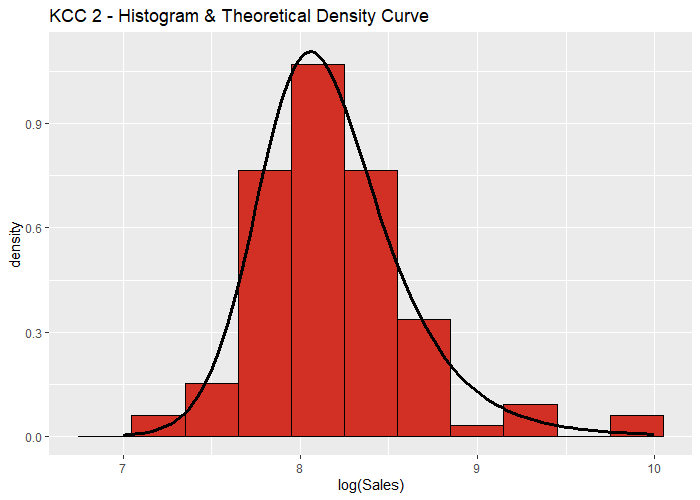
\includegraphics[width=\linewidth]{figures/kcc_2_density.png}
  \caption{Histogram \& theoretical density}
  \label{fig:kcc_2_density}
\end{subfigure}
\begin{subfigure}{.45\textwidth}
  \centering
  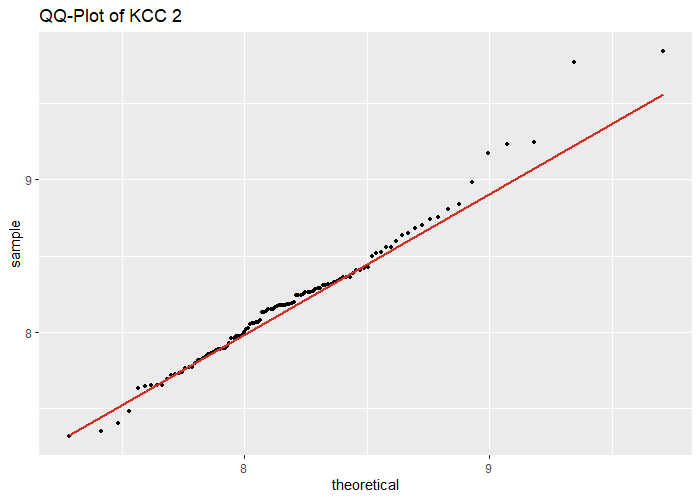
\includegraphics[width=\linewidth]{figures/kcc_2_qqplot.png}
  \caption{QQ-Plot}
  \label{fig:kcc_2_qqplot}
\end{subfigure}
\caption{exGaussian distribution fitted to log-sales of \ac{KCC} 2}
\label{fig:kcc_2_marginal}
\end{figure} 




\begin{figure}[H]
\centering
  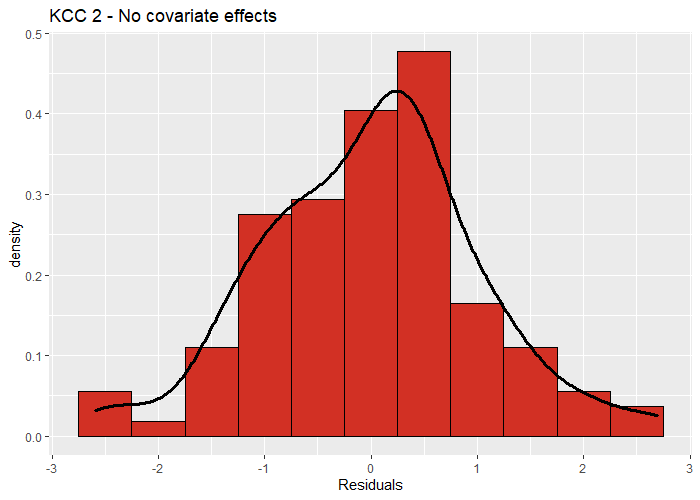
\includegraphics[width=0.45\linewidth]{figures/res_kcc_2_no_covariates.png}
  \caption{Residuals of KCC 2 log-sales fitted to an exGaussian distribution with no covariate effects together with their density curve}
  \label{fig:res_kcc_2_no_covariates}
\end{figure}

As can be seen in \autoref{fig:res_kcc_2_no_covariates}, the residuals of the fitted distribution are not too far from a normal distribution. 
In fact, a Shapiro-Wilk normality test (see \ref{ssec:shapiro_wilk}) will fail to reject the null hypothesis, returning a p-value of 0.6645.
There still exist skewness in the distribution of the residuals and correction will be attempted in the following. \\

The findings so far indicate that the overall fit for this cluster are quite satisfiable and also support interpretability of the estimated parameters. \\
To make the estimation more precise and to get a better understanding of what is driving sales, flexible estimation of the distribution parameters is required and thus covariate effects shall be included. \\
%The temporal effects in particular are of special interest. 

After multiple equation setups for the marginal distribution of \ac{KCC} 2, the chosen \ac{GAMLSS} model specification (see Section \ref{ssec:gamlss}) is as follows:

\begin{equation}
\begin{aligned}
\mu &= \beta_{01} + f_{11}(\textit{time}) + f_{12}(\textit{total\_markdown\_pct}) \\ \noalign{\vskip5pt}
log(\sigma) &= \beta_{02} + f_{21}(\textit{time}) \\ \noalign{\vskip5pt}
log(\nu) &=  \beta_{03}, 
\end{aligned}
\label{eq:gamlss_kcc_2}
\end{equation} \\
where the smooth functions $f_{11}$, $f_{21}$ are P-Splines with 20 knots each and $f_{12}$ is again a smooth function build by P-Splines with 10 knots. For the scale and shape parameters ($\sigma$ and $\nu$ respectively) the logarithmic link function is used to ensure that they are mapped to the real positive line as the exGaussian distribution family can only express positive skewness ($\nu$). \\

The absence of the Black Friday and Friends \& Family components in model \ref{eq:gamlss_kcc_2} is due to the fact that the effects of activated promotions to the expected sales are negative, which is contradictory to the analysis made earlier in Chapter \ref{ssec:grouped_patterns}. The output after excluding those indicator variables seem to be more stable as and intuitive.\footnote{This might be traced back to the fact that promos obviously yield higher markdowns and thus we reach redundancy of variables in the model.}















